% !TEX root = ../Masterarbeit.tex
\chapter{Grundlagen \& Definitionen}
In diesem Kaptiel werden die Grundlagen beschrieben, auf die der Hauptteil aufbaut. Zudem behandelt das Kapitel die Begriffsbestimmung und die genauen Eigenschaften reaktiver Systeme. Da die Umsetzung reaktiver Systeme gewisse Programmierparadigmen vorausgesetzt, werden diese nach den reaktiven Merkmalen erklärt.

\section{Eigenschaften reaktiver Systeme}
Reaktive Anwendungen haben die Eigenschaften folgendes zu leisten bzw. folgende Punkte zu erfüllen~\cite[S.~19ff]{kuhn_reactive_2015}~\cite[S.~6]{vernon_reactive_2016}.\\
Eine reaktive Anwendung muss\ldots
\begin{enumerate}
\item \ldots auf variable Belastung reagieren (siehe~\fullref{subsec:elastic}). Das System ist automatisch in der Lage dynamische Skalierung durchzuführen und nicht benötigte Ressourcen wieder freizugeben.
\item \ldots auf Fehler reagieren (siehe~\fullref{subsec:resilient}). Die Software ist von Grund auf widerständsfähig gegenüber Fehlerzuständen. Die Wiederherstellung des Normalzustand erfolgt automatisch.
\item \ldots auf Nutzer oder Komponenten reagieren (siehe~\fullref{subsec:responsive}). Jede Anfrage wird in der geforderten Antwortzeit oder schneller bearbeitet.
\item \ldots auf Nachrichten reagieren (siehe~\fullref{subsec:messagedriven}). Das System verwendet asynchrone Nachrichtenübertragung zur Kommunikation zwischen Komponenten.
\end{enumerate}

Die nachfolgenden Abschnitte erklären die Merkmale im Detail und zeigen den Zusammenhang zwischen ihnen.

\subsection{Elastic}\label{subsec:elastic}
Eine reaktive Anwendung muss auf variable Belastung ebenso variabel bzw. dynamisch reagieren können. Wird beispielsweise ein Online Shop in einer Fernsehwerbung oder von einem bekannten Blog erwährt, müssen kurzfristig sehr viele Anfragen angemessen und zufriedenstellend verarbeitet werden~\cite[S.~39]{kuhn_reactive_2015}. Überdies muss davon ausgegangen werden, dass die Nutzerzahlen oder auch die Anforderungen bzgl. Antwortzeiten zukünfigt steigen.\\
Folglich muss ein System dazu in der Lage sein zu skalieren. Selbst durch vertikale Skalierung, also dem Hinzufügen von weiteren Ressourcen zu einem Host, stößt man aufgrund der schnell steigenden Anforderungen in kurzer Zeit an die Grenzen eines einzelnen Hosts. Dementsprechend muss ein System nicht nur vertikal, sondern auch horizontal skalieren können. Dazu werden Anwendungen auf einem Computercluster, einem Verbund aus mehreren Hosts bzw. Nodes, verteilt~\cite[S.~7]{vernon_reactive_2016}. Bei der horizontalen Skalierung werden dem Computercluster weitere Nodes hinzugefügt.\\
Es ist deshalb wichtig, die Teilaufgaben einer Applikation zu identifizieren und auf einzelne Komponenten aufzuteilen. Die Komponenten müssen lose gekoppelt sein, um sie wie bereits erwähnt auf einzelne Nodes verteilen zu können~\cite[S.~40]{kuhn_reactive_2015}.\\
Das Reactive Manifesto fordert zudem auch, das System so zu gestalten, dass es \enquote{Scaling down} fähig ist. Das bedeutet ungenutze und nicht benötigte Ressourcen müssen wieder freigegeben werden. Dadurch kann man ein hochskalierbares und reaktives System kosteneffizient betreiben. Im Reactive Manifesto hat man sich auf den Begriff \textit{elastic} geeinigt, um deutlich zu machen, dass man in beide Richtungen skalieren kann. Bei reaktiven Applikationen spricht man deshalb von elastischer bzw. dynamischer Skalierung~\cite[S.~8]{vernon_reactive_2016}. Für die Software bedeutet dies, dass einzelne Nodes jederzeit hinzugefügt und entfernt werden können.\\
In Folge dessen werden Komponenten ebenso dynamisch auf verschiedene Nodes verteilt. Insofern dürfen die Komponenten und deren Kommunikation nicht von einem physikalischen Host oder anderen \enquote{örtlichen} Gegebenheiten abhängig sein~\cite[S.~8]{vernon_reactive_2016}. Diese Eigenschaft wird \enquote{\gls{locationtransparency}} genannt.\\

Um die Leistungsfähigkeit einer Anwendung zu berechnen, kann auf das Gesetz von John Little (\enquote{Little's Law}) zurückgeriffen werden. Das Gesetz besagt, dass die durchschnittliche Anzahl von Anfragen $L$ gleich dem Produkt der durchschnittlichen Anfragerate $\lambda$ und ihrer durchschnittlichen Bearbeitungsdauer $W$ ist.

\begin{figure}[H]
  \[L := \lambda W\]
  \caption{Berechnung der Leistungsfähigkeit mithilfe von \enquote{Little's Law}}
\end{figure}

Angenommen eine Anwendung benötigt für die Bearbeitung einer Anfrage $10ms$ und im Durchschnitt empfängt die Anwendung eine Anfrage pro Sekunde. 

\begin{figure}[H]
  \[L := \lambda W = \frac{1}{1s} 10ms = 0.01\]
\end{figure}

\vspace{-0.5cm}

Das Gesetz von Little besagt, dass die durchschnittliche Anzahl von nebenläufigen Anfragen $0.01$ entspricht. Folglich sind die Anforderungen sehr gering und die Anwendung muss im Durchschnitt nur eine Anfrage zur selben Zeit bearbeiten. Steigt jedoch die Anzahl der Anfragen auf 500 pro Sekunde oder gar 1000 pro Sekunde müssen entsprechend 5 oder 10 Anfragen im Durchschnitt parallel verarbeitet werden können.\\
Mit dem Gesetz von Little können die Voraussetzungen für die Leistungsfähigkeit einer Anwendung im Vorfeld betrachtet werden. Zudem eignet sich das Gesetz dazu eine dynamische Skalierung zur Laufzeit vorzunehmen. Hierfür ist ein stetiges Monitoring der eingehenden Anfragen und der Bearbeitungsdauer notwendig. Jedoch sollte beachtet werden, dass die dynamische Skalierung auf einer Cloud Plattform schnell teuer werden kann --- beispielsweise durch einen \gls{denialofservice}.

\pagebreak

\subsection{Resilient}\label{subsec:resilient}
Eine Software \textit{resilient} zu entwickeln bedeutet nicht, dass die Software fehlerfrei ist. Es bedeutet, dass die Software sich von einem Fehlerzustand erholen kann~\cite[S.~6]{vernon_reactive_2016}.\\
Schon bei dem Entwurf von Software wird versucht Fehler von vornherein zu bedenken und mit ihnen sinnvoll umzugehen. Folgendes Zitat von Jonas Bonér macht deutlich, wie wichtig die Widerstandsfähigkeit einer Software ist:

\begin{quotation}
Without resilience, nothing else matters. If your beautiful, production-grade, elastic, scalable, highly concurrent, non-blocking, asynchronous, highly responsive and performant application isn't running, then you're back to square one. It starts and ends with resilience.~\citetext{Bonér, Jonas; 2015}
\end{quotation}

Im Grunde ist diese Aussage trivial. Eine Software, die nicht läuft ist unbrauchbar --- egal wie komplex und durchdacht die Architektur auch sein mag.\\
Es ist aber nicht nur die eigene Software, die betroffen sein kann. Andere externe Softwarekomponenten, von denen man abhängt, oder auch die Hardware, kann im laufenden Betrieb Probleme bereiten~\cite[S.~33]{kuhn_reactive_2015}.\\
Der Schluss, den man daraus ziehen sollte, lautet deshalb nicht, ob ein Fehler auftritt, sondern viel mehr wann und wie häufig das passiert. Für den Benutzer ist es nebensächlich, warum ein interner Fehler aufgetreten ist. Die Anwendung wird in diesem Moment nicht das tun, was der Benutzer von ihr erwartet~\cite[S.~33]{kuhn_reactive_2015}.\\

Im Reactive Manifesto hat man für dieses Problem bzw. die Eigenschaft ganz bewusst den Begriff \textit{resilience}, also zu Deutsch Widerstandfähigkeit und nicht Ausfallsicherheit gewählt. Man möchte deutlich machen, dass es nahezu unmöglich ist, ein ausfallsicheres System zu schaffen. Deshalb setzt man auf widerstandsfähige Systeme, welche mit Fehlerzuständen sinnvoll umgehen und sich vor allem von diesen wieder erholen. Folglich ist ein reaktives System nicht nur fehlertolerant, sondern geht noch einen Schritt weiter~\cite[S.~34]{kuhn_reactive_2015}.\\

Um die Eigenschaft \textit{resilience} zu erfüllen, muss das System in Komponenten aufgeteilt und anschließend verteilt werden. Zusätzlich ist es notwendig, die verteilten Komponenten voneinander abzuschotten~\cite[S.~34]{kuhn_reactive_2015}~\cite[S.~7]{vernon_reactive_2016}.\\
Aufgrund der verteilten und abgeschotteten Komponenten können Fehler isoliert werden. Hierfür führt man das Prinzip der \enquote{Supervision} ein. Nach- bzw. untergeordnete Komponenten informieren ihren Supervisor im Falle eines Fehlers. Dieser hat nun die Möglichkeit die Subkomponente z.B. neuzustarten oder eine erneute Anfrage zustellen. 

\subsection{Responsive}\label{subsec:responsive}
Eine reaktive Anwendung muss zu jederzeit auf jede Anfragen reagieren. Das heißt, die Anwendung ist jederzeit \textit{responsive}. Anfragen können nicht nur durch einen Benutzer ausgelöst werden, sondern können auch von anderen Diensten oder Komponenten initiiert werden. Als Client einer reaktiven Anwendung muss man sich darauf verlassen können, dass eine Antwort in einem festgelegten Zeitraum eintrifft. Das bedeutet es müssen Timeouts festgelegt werden, nach denen eine langwierige Anfrage für fehlerhaft erklärt wird. Auch für die interne Kommunikation müssen Timeouts definiert werden.\\
Ist eine Anwendung nicht \textit{elastic} (siehe~\ref{subsec:elastic}) und/oder nicht \textit{resilient} (siehe~\ref{subsec:resilient}), kann sie auch nicht \textit{responsive} sein. Eine reaktive Anwendung muss unter Last skalieren, um die geforderte maximale Antwortzeit einzuhalten oder einen Systemausfall zu vermeiden. Gleichzeitig eingehende Anfragen müssen parallel verarbeitet werden können und dürfen nicht von langsamen Anfragen blockiert werden. Fallen Komponenten aus, z.B. durch einen Hardwarefehler, könnten diese aufgrund der \gls{locationtransparency} auf einem anderen Node neu gestartet werden, um die \textit{responsiveness} aufrechtzuerhalten.

\pagebreak

\subsection{Message-driven}\label{subsec:messagedriven}
Um die bereits erwähnten Eigenschaften \textit{elasticity} (\ref{subsec:elastic}), \textit{resilience} (\ref{subsec:resilient}), sowie die daraus folgende \textit{responsiveness} (\ref{subsec:responsive}) zu erfüllen, müssen reaktive Anwendungen \textit{message-driven} sein~\cite{webber_what_2014}~\cite[S.~43]{kuhn_reactive_2015}. Die Basis einer reaktiven Anwendung ist somit die vierte Eigenschaft aus dem Reactive Manifesto~\cite{boner_reactive_2014}.\\
Ist ein System \textit{message-driven}, erfolgt die Kommunikation ausschließlich über asynchronen Nachrichtenaustausch zwischen den Komponenten, wodurch eine strikte Abgrenzung der Komponenten erfolgt. Durch die Abstraktion der Kommunikation wird eine lose Kopplung zwischen den Komponenten sichergestellt. Darüber hinaus sind die Komponenten voneinander isoliert, wodurch es möglich ist, Fehler als Nachrichten zu delegieren (siehe~\ref{subsec:resilient}). Durch den expliziten Nachrichtenaustausch kann über \glspl{messagequeue} und \gls{flowcontrol} die Last verteilt und kontrolliert werden. Ebenso wird die gewünschte \gls{locationtransparency} durch die Entkopplung über den asynchronen Nachrichtenaustausch ermöglicht~\cite{boner_reactive_2015}~\cite[S.~43]{kuhn_reactive_2015}.\\

Folglich ist die reaktive Eigenschaft \textit{message-driven} zwingend erforderlich und nicht nur ein Detail der Implementierung. Auf den Unterschied zwischen synchroner und asynchroner Kommunikation wird später nochmals eingegangen (siehe \ref{subsec:communication}).\\

Die folgende Abbildung \ref{fig:four-traits} verdeutlicht den Zusammenhang der vier Eigenschaften des Reactive Manifestos. Neben dem wohl wichtigsten Ziel der \textit{responsiveness} hat die reaktive Architektur weitere Vorteile, wie beispielsweise Wartbarkeit und Erweiterbarkeit. Jedoch werden diese weiteren Vorteile nur in der Einleitung des Reactive Manifestos beschrieben und nicht als Kerneigenschaft formuliert~\cite{boner_reactive_2014}. Die Ziele erreicht man durch die Eigenschaften \textit{elasticity} und \textit{resilience}. Die Grundvoraussetzung ist im wesentlichen die asynchrone, nicht-blockierende und nachrichtengetriebene Kommunikation, welche durch die Eigenschaft \textit{message-driven} ausgedrückt wird.

\pagebreak

Man kann argumentieren, dass auch traditionelle Software Architekturen \textit{responsiveness}, Wartbarkeit und Erweiterbarkeit zum Ziel haben. Jedoch werden dabei die für heutige Anforderungen wichtigen Eigenschaften \textit{elasticity} und \textit{resilience} vernachlässigt oder ignoriert.

\begin{figure}[H]
 \centering
 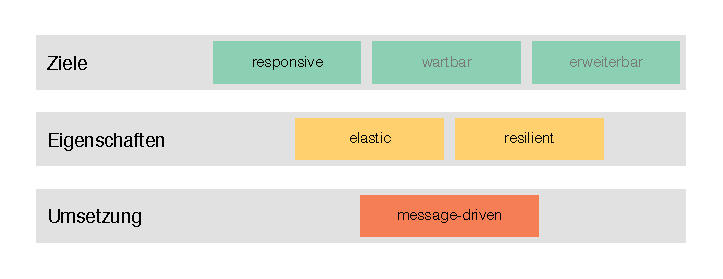
\includegraphics[width=1.0\textwidth]{3-Grundlagen/four-traits/four-traits.eps}
 \caption{Die vier Merkmale einer reaktiven Anwendung \cite{kuhn_code_2015}}
 \label{fig:four-traits}
\end{figure}

\pagebreak

\section{Parallelität \& Concurrency}

\subsection{Notwendigkeit}\label{subsec:notwendigkeit}
Die Prozessorhersteller sind in den letzten Jahren an gewisse Grenzen bei der Entwicklung von CPUs gestoßen. Seit 2003 stagniert die Entwicklung hinsichtlich der Taktraten von Prozessoren. Die Beobachtungen von Gordon Moore (\enquote{Moore's Law}) scheinen nach wie vor ihre Gültigkeit zu haben und die Zahl der Transistoren verdoppelt sich ungefähr alle zwei Jahre. Diese werden jedoch nicht genutzt, um eine einzelne CPU schneller zu machen. Hersteller setzen stattdessen seit einigen Jahren auf Multicore-Architekturen~\cite[S.~1]{butcher_seven_2014}~\cite[S.~108]{vernon_reactive_2016}~\cite{sutter_free_2004}.\\
Herb Sutter veröffentlichte diesbezüglich 2004 einen Artikel mit dem Titel \enquote{The free lunch is over}. Mit \enquote{free lunch} bezog er sich auf die Tatsache, dass sequenzielle Anwendungen ohne das Zutun von Entwicklern aufgrund der damals noch steigenden Taktraten schneller wurden --- vielmehr schneller ausgeführt wurden.\\
Im Hinblick auf die Multicore-Prozessoren und der mehr oder weniger stagnierenden Taktraten müssen Anwendungen ihre Aufgaben und Teilaufgaben nebenläufig und parallel ausführen, um die heutigen und zukünftigen Prozessoren optimal auszulasten~\cite[S.~45]{kuhn_reactive_2015}~\cite{sutter_free_2004}~\cite[S.~1]{butcher_seven_2014}.\\
Sequenzielle Programme werden Schritt für Schritt ausgeführt. Genauer gesagt, erfolgt die Ausführung der einzelnen Befehle nach einer vorgegebenen Reihenfolge. Folglich profitiert ein sequenzielles Programm nicht vollumfänglich von modernen Multicore-Prozessoren. Hier kommen nun \gls{concurrency} (dt. Nebenläufigkeit) und Parallelität ins Spiel~\cite[S.~3]{butcher_seven_2014}.\\

Die Welt, in der wir leben, ist hochgradig parallel. Während wir Menschen mit dem Auto über eine Autobahn fahren, nehmen wir, wenn auch meist nur unterbewusst, viele unterschiedliche Dinge gleichzeitig wahr. Während wir uns sportlich betätigen, hören wir meistens gleichzeitig zum Laufen Musik, um uns anzuspornen.\\

Während wir zum Zeitvertreib auf unserem Smartphone ein Spiel spielen, kann es derweil trotzdem E-Mails abrufen. Würden diese Prozesse streng sequenziell und nicht parallel ablaufen, hätten wir vermutlich schon längst hunderte Autounfälle in unserem Leben verursacht. Es wäre fatal, wenn der Mensch Bewegungen nur bewusst vollziehen könnte.\\
Blickt man nun auf Parallelität im Bezug auf Prozessoren und Software, wird zwischen mehreren Ebenen von Parallelität unterschieden. Zum Beispiel kann ein Singlecore-Prozessor, aufgrund von Technologien wie \gls{pipelining}, mehrere Schritte parallelisieren. Ebenso sind \gls{multitasking} Betriebssysteme in der Lage auf einem Singlecore-Prozessor mehrere Prozesse nebenläufig bzw. quasi-parallel auszuführen~\cite[S.~3~\&~S.~4]{butcher_seven_2014}. Der folgende Abschnitt bezieht sich auf Parallelität in Bezug auf Multicore-Prozessoren und wie diese erreicht werden kann.\\
\gls{concurrency} und Parallelität werden fälschlicherweise oft als Synonyme verwendet. Die beiden Begriffe sind verwandt, beschreiben jedoch verschiedene Sachverhalte. Aus der Sicht eines Problems (Problemdomäne), bedeutet \gls{concurrency} das Bearbeiten gleichzeitig oder annähernd gleichzeitig eintreffender Ereignisse. Im Gegensatz dazu bezieht sich Parallelität auf die beschleunigte Lösung eines Problems durch Fragmentierung und der simultanen Bearbeitung der Teilprobleme~\cite[S.~1~\&~S.~2]{butcher_seven_2014}~\cite[S.~15]{vernon_reactive_2016}.\\
Rob Pike formulierte den Unterschied zwischen \gls{concurrency} und Parallelität wie folgt:

\begin{quotation}
  Concurrency is about dealing with lots of things at once. Parallelism is about doing lots of things at once. [...] Concurrency provides a way to structure a solution to solve a problem that may (but not necessarily) be parallelizable~.
\cite[S.~10]{pike_concurrency_2012}
\end{quotation}

Im Grunde bedeutet das, die \gls{concurrency} beschreibt die Koordination mehrerer unabhängiger Abläufstränge (Threads) --- die nicht zwangsläufig simultan ausgeführt werden. Parallelität bedeutet hingegen die simultane bzw. gleichzeitige Ausführung von Berechnungen~\cite[S.~8-9]{pike_concurrency_2012}~\cite[S.~3]{butcher_seven_2014}.\\

Kann ein Problem nebenläufig beschrieben bzw. entworfen werden, ist es möglich, die Anwendung parallel und entsprechend effizienter auszuführen~\cite[S.~19~\&~S.~30]{pike_concurrency_2012}.\\

Die effizientere Ausführung hat jedoch Grenzen und diese hängen von den sequenziellen Segmenten ab. Gene Amdahl stellte hierfür bereits 1967 ein Modell auf (\enquote{Amdahl's Law}), welches den Grad der Beschleunigung einer Anwendungen durch dessen parallele Anteile beschreibt. So zum Beispiel kann eine Anwendung, die nur zu 90~\% parallelisiert ist, maximal um den Faktor 10 schneller ausgeführt werden~\cite{amdahl_validity_1967}.\\
Die sequenziellen respektive synchronisierten Abschnitte erfordern, dass sich die Ausführungseinheiten --- spricht Kerne eines Multicore-Prozessors --- abstimmen. Amdahl's Law ignoriert den Aufwand dieser Koordination. Die Universal Scalability Law rechnet den Faktor der Koordinationskosten mit ein und ist somit der wirklichkeitsnähere Ansatz. Ab einer gewissen Anzahl von Ausführungseinheiten führt eine erneute Erhöhung der Anzahl nicht zu einer Beschleunigung der Ausführung sondern hat den gegenteiligen Effekt \cite[S.~46]{kuhn_reactive_2015}.\\
Beide Modelle zeigen, wie wichtig es ist, auf sequenzielle Abschnitte zu achten und diese möglichst zu vermeiden.\\

Die Art und Weise, wie wir heute mit der digitalen Welt interagieren, ist nebenläufig und parallel. Demnach müssen Anwendungen ebenso nebenläufig sein, um den Anforderungen zu entsprechen~\cite[S.~5]{butcher_seven_2014}~\cite[S.~3~\&~S.~178]{armstrong_programming_2013}.\\
Ein nebenläufiges Design erlaubt es einer Anwendung \textit{responsive}, fehlertolerant und effizient zu sein~\cite[S.~4~\&~S.~6]{butcher_seven_2014}~\cite[S.~6]{armstrong_programming_2013}. Nur eine Anwendung, die nebenläufig mehrere Ereignisse verarbeiten kann, ist in der Lage \textit{responsive} zu sein.

\pagebreak

 Beispielsweise kann ein Browser mehrere Webseiten gleichzeitig (nebenläufig) laden und der Benutzer hat die Möglichkeit währenddessen eine weitere Seite zu öffnen, ohne auf die Beendigung der anderen Ladevorgänge warten zu müssen. Verteilt man eine Anwendung auf mehrere Nodes, muss diese implizit nebenläufig sein --- oder anders ausgedrückt, nebenläufiges Design erlaubt das Verteilen auf mehrere Nodes. Die Möglichkeit eine Anwendung zu verteilen und somit redundant zu betreiben, ist Basis für \textit{resilience} und \textit{elasticity}~\cite[S.~6]{butcher_seven_2014}~\cite[S.~6~\&~S.~7]{armstrong_programming_2013}.\\

Zusammenfassend kann man diesem Abschnitt entnehmen, dass reaktive Anwendungen per Definition nebenläufig entworfen und umgesetzt werden müssen, um die Eigenschaften des Reactive Manifestos zu erfüllen.

\pagebreak

\subsection{Share nothing}\label{subsec:sharenothing}
Nebenläufige Komponenten nutzen traditionellerweise gemeinsame bzw. geteilte Datenstrukturen (\enquote{Shared State}), um zu interagieren und zu kommunizieren. Folglich kann der Zugriff auf diese Daten nebenläufig und parallel erfolgen. Aus diesem Grund müssen die Operationen synchronisiert werden. Hierfür nutzt man das Konzept der \enquote{\gls{mutualexclusion}}. Man stellt beispielsweise über Locks sicher, dass nur ein Thread zur selben Zeit auf die Daten zugreifen kann~\cite[S.~10]{butcher_seven_2014}. Der Zugriff auf die Daten erfolgt somit sequenziell. Die Erkenntnisse durch Amdahl's Law oder der Universal Scalabilty Law (\ref{subsec:notwendigkeit}) zeigen, dass die Vorteile einer nebenläufigen Anwendung an dieser Stelle zunichtegemacht werden~\cite[S.~45]{kuhn_reactive_2015}. Zudem haben Anwendungen mit Shared State unter anderem mit Problemen wie \gls{memorycorruption}, \glspl{deadlock} und \gls{starvation} zu kämpfen~\cite[S.~117]{vernon_reactive_2016}.\\
Neben Locks gibt weitere Algorithmen um \gls{mutualexclusion} effizienter umzusetzen und Shared State zu ermöglichen. Locks haben den Nachteil, dass Threads zeitweilig blockiert bzw. zurückgehalten werden, wenn bereits ein anderer Thread den synchronisierten Teil --- also den kritischen Abschnitt --- ausführt. Beispielsweise können mithilfe von \enquote{Optimistic Locks} und atomaren \enquote{Compare and Swap} Operationen kritische Abschnitte ohne blockierende Locks umgesetzt werden. Die Erklärung der Algorithmen im Rahmen dieser Arbeit wäre nicht zielführend. Denn diese Algorithmen sind meist schwer zu implementieren und in Folge dessen ist deren Umsetzung meist fehlerbehaftet \cite{jenkov_non-blocking_2015}. Laut Martin Thompson et al. haben selbst \enquote{Compare and Swap} Operationen einen gewissen Koordinationsaufwand der nicht zu vernachlässigen ist \cite{thompson_disruptor_2011}.\\
Darüber hinaus ist zu erwähnen, dass in einem verteilten System diese Algorithmen aufgrund der Netzwerkkommunikation schwer umzusetzen sind \cite[S.~45]{butcher_seven_2014}.\\

\pagebreak

In reaktiven Anwendungen müssen Komponenten voneinander isoliert sein, um die Eigenschaften \textit{elastic} und \textit{resilient} erfüllen zu können. Folglich können die Komponenten auch keine Informationen teilen respektive Shared State besitzen --- kurz das Share nothing Prinzip.\\
Um mit einer anderen Komponente zu interagieren, müssen reaktive Komponenten asynchrone Nachrichten austauschen (\ref{subsec:messagedriven}).\\
Dieses Konzept der nebenläufigen Interaktion ist eine Alternative zu den geteilten Datenstrukturen. Der Vorteil ist, dass Informationen und somit auch Aufgaben nur durch den expliziten Nachrichtenaustausch übermittelt und nicht geteilt werden. Man benötigt keine \gls{mutualexclusion} und kann effizient nebenläufige Aufgaben abarbeiten \cite[S.~439]{armstrong_programming_2013}. In einem späteren Abschnitt werden zwei reaktive Concurrency Modelle (\ref{sec:concurrency-models}) vorgestellt, die dieses Prinzip umsetzen.\\

Durch die lose Kopplung erhält man klare Grenzen zwischen den Komponenten. Dies führt zur Kapselung von Fehlern, Implementierungsdetails und Verantwortlichkeiten. Des Weiteren hilft es bei der Umsetzung von \gls{locationtransparency} und der effizienteren Nutzung der bereitgestellten Ressourcen~\cite[S.~45]{kuhn_reactive_2015}.

\pagebreak

\subsection{Kommunikation \& Interaktion}\label{subsec:communication}
Eine reaktive Anwendung ist \textit{message-driven}. Hierzu müssen Nachrichten zwischen den Komponenten ausgetauscht werden. Es gibt zwei Möglichkeiten der Kommunikation. Zum einen die synchrone und zum anderen die asynchrone Kommunikation.

\subsubsection{Synchrone Kommunikation}
Die traditionelle Kommunikation zwischen zwei Komponenten ist die synchrone Kommunikation. Komponente \textit{A} ruft eine Funktion \textit{f} der Komponente \textit{B} auf. Die Berechnung erfolgt synchron und deshalb wartet Komponente \textit{A} auf das Ergebnis und kann dann erst die weiteren Schritte sequenziell abarbeiten. Die weiteren Schritte müssen jedoch nicht von dem Ergebnis der Funktion \textit{f} abhängig sein und trotzdem wird deren Berechnung blockiert. Sollte bei dem Funktionsaufruf ein Fehler auftreten, werden die nachfolgenden Befehle nicht ausgeführt. Die Komponente \textit{B} ist von diesem Fehler ebenfalls betroffen, solange die beiden Komponenten im gleichen Thread ausgeführt werden. Folglich sind die Komponenten \textit{A} und \textit{B} stark voneinander abhängig~\cite[S.~22]{kuhn_reactive_2015}~\cite{jackson_how_2016}.\\
Es wird klar, dass diese Art der Kommunikation für \textit{responsivness}, \textit{resilience} und \textit{elasticity} nicht förderlich ist~\cite[S.~46]{kuhn_reactive_2015}.

\subsubsection{Asynchrone Kommunikation}
Sobald die Komponenten \textit{A} und \textit{B} verteilt werden, löst sich die angesprochene Kopplung. Dies kann durch Ausführung in jeweils eigenen Threads geschehen oder durch die Verteilung auf mehrere Nodes. Dies ist ein notwendiger Schritt hin zu einer reaktiven Anwendung~\cite[S.~22]{kuhn_reactive_2015}.\\
Innerhalb verteilter Anwendungen ist synchrone Kommunikation (in seiner einfachsten Form ein Funktionsaufruf), wie bereits erwähnt, nicht wünschenswert. Oft werden die Gegebenheiten lokaler Funktionsaufrufe auf eine verteile Netzwerkkommunikation übertragen. Peter Deutsch formulierte diesbezüglich sieben Irrtümer bzw. Annahmen, die im Bezug auf verteile Systeme gemacht werden.\\

Zum Beispiel die Annahme ein Netzwerk wäre ausfallsicher oder die Latenz der Netzwerkkommunikation geht gegen Null. Diese Annahmen treffen selbstverständlich nicht zu~\cite[S.~1]{rotem_fallacies_2008}. In einem weiteren Artikel beschäftigen sich Waldo et al. ebenfalls mit der Kommunikation in einem verteilten System und kommen zu dem Schluss, dass vor allem unvorhersehbare Latenz und teilweiser Ausfall der Kommunikation unvermeidbar sind~\cite{waldo_note_1994}.\\
Im Gegensatz zur synchronen Kommunikation führt der Sender bei einer asynchronen Kommunikation seine Aktivitäten und Berechnungen fort und wartet nicht auf die Empfangsbestätigung oder Antwort des Empfängers. Der Empfänger selbst verarbeitet die Nachrichten meist auch asynchron. Eingehende Nachrichten werden zuerst in einer \gls{messagequeue} bis zur Bearbeitung zwischengelagert. Man spricht auch von asynchroner und nicht blockierender Kommunikation. Durch die asynchrone Programmierung werden die Ressourcen nicht durch unvermeidbares Warten blockiert sondern effektiver genutzt~\cite[S.~48]{kuhn_reactive_2015}.\\

Aufgrund des Share nothing Prinzips (siehe~\ref{subsec:sharenothing}) sollten Komponenten über Nachrichten miteinander interagieren. Der Abschnitt hat gezeigt, dass diese Interaktion asynchron und nicht blockierend ablaufen sollte, um die Ressourcen effizient zu nutzen~\cite[S.~48~\&~S.~49]{kuhn_reactive_2015}.

\pagebreak

\section{Funktionale Programmierung}
Die funktionale Programmierung ist ein Programmierparadigma, bei dem die Anwendungen ausschließlich aus Ausdrücken bzw. Funktionen bestehen. Zudem werden Funktionen bevorzugt, die keine Seiteneffekte besitzen und deshalb \enquote{Pure Functions} genannt werden. Funktionen werden darüber hinaus wie übliche Datenstrukturen (z.B. Integer oder Boolean) behandelt und können Variablen zugewiesen oder als Argument übergeben werden. In funktionalen Programmiersprachen haben Funktionen somit den gleichen Stellenwert, wie auch andere Datentypen. Man spricht deshalb von sogenannten \enquote{First-class Functions}~\cite[S.~50]{butcher_seven_2014}~\cite[S.~3~\&~S.~19]{chiusano_functional_2015}.\\
Folgende Abschnitte erklären gewisse Grundkonzepte der funktionalen Programmierung und machen ihren Bezug zu reaktiven Anwendungen deutlich. 

\subsection{Immutable}
In der imperativen Programmierung wird meist von den so genannten veränderbaren Zuständen Gebrauch gemacht (engl.~\enquote{Mutable State}). Ein veränderbarer Zustand ist eine Variable, die jederzeit modifiziert werden kann. Im Abschnitt zu \fullref{subsec:sharenothing} wurde bereits deutlich gemacht, dass veränderbarer und geteilter Speicher (engl. \enquote{Shared Mutable State}) bei nebenläufigen Anwendungen zu verschiedenen Problemen führen kann. Die funktionale Programmierung versucht \enquote{Mutable State} von vornherein zu verhindern~\cite[S.~50]{butcher_seven_2014}.\\
Ist eine Variable \enquote{immutable} bedeutet das, sie ist nach dem initialen Setzen eines Wertes nicht mehr veränderbar. Der gleichzeitige Zugriff auf einen \enquote{Shared Immutable State} muss somit nicht mehr synchronisiert werden, da die Variable nur einmal beschrieben werden kann~\cite[S.~50]{butcher_seven_2014}~\cite[S.~62]{kuhn_reactive_2015}.\\

\pagebreak

\subsection{Pure Functions}
Die Pure Functions sind Funktionen ohne Seiteneffekte. Eine Pure Function liefert bei gleicher Eingabe auch immer das gleiche Ergebnis~\cite[S.~61]{kuhn_reactive_2015}. Eine Funktion, die eine global definierte Zählvariable inkrementiert, hat somit Seiteneffekte. Desweiteren darf eine Pure Function keine höheren Datentypen, wie Objekte oder Listen verändern. Auch der Zugriff auf Netzwerk oder Dateisystem gilt als Seiteneffekt~\cite[S.~3]{chiusano_functional_2015}~\cite[S.~62]{kuhn_reactive_2015}.
Der Vorteil von Pure Functions ist, dass der Aufruf durch das Ergebnis ersetzt werden kann. Verallgemeinert man dieses Prinzip auch auf Ausdrücke, spricht man von der sogenannten \enquote{Referential Transparency}~\cite[S.~9]{chiusano_functional_2015}~\cite[S.~62]{kuhn_reactive_2015}. Folgendes Beispiel zeigt eine Funktion, die zwei Zahlen addiert (\ref{lst:lst1}). Diese Funktion ändert keine bestehenden Variablenwerte und hat auch sonst keinerlei Seiteneffekte. Der Aufruf dieser Funktion kann folglich mit dem Ergebnis ersetzt werden, wie die letzte Zeile des Beispiels zeigt.

\begin{lstlisting}[caption={Beispiel für eine Pure Funcition},label={lst:lst1}]
def add(a: Int, b: Int): Int = {
  return a + b
}

add(add(1, 2), add(3, 4))
// = (1 + 2) + (3 + 4) = 10

add(3, 7)
// = 3 + 7 = 10
\end{lstlisting}

Dieses einfache Beispiel nutzt wiederum eine Pure Function, die bereits durch die Programmiersprache, in diesem Fall Scala, bereitgestellt wird. Die Addition zweier Zahlen durch den \textit{+} Operator. Auch in nicht funktionalen Sprachen gibt es viele Ausdrücke und Pure Functions, die die Referential Transparency wahren. Zum Beispiel die mathematischen Operatoren oder die Funktion zur Bestimmung der Länge einer immutable Zeichenkette --- meist \textit{length} genannt.\\

Ein weiteres Beispiel für die Referential Transparency sind Funktionen, die einen bestehenden Wert kopieren und bei diesem Vorgang Veränderungen durchführen ohne den alten Wert bzw. die alte Referenz zu verändern (siehe~\autoref{lst:lst2}).

\begin{lstlisting}[caption={Beispiel einer Funktion mit Referential Transparency.},label={lst:lst2}]
def moveX(p: Point, x: Int): Point = {
  return new Point(p.x + x, p.y)
}
val p1 = new Point(1, 1)
val p2 = moveX(p1, 2)
// p1 = new Point(1, 1)
// p2 = new Point(3, 1)
\end{lstlisting}

Die Funktion \textit{moveX} verändert den übergebenen Wert \textit{p} nicht, sondern kopiert bestehende Variablen des Typs und verändert diese. Der Wert von \textit{p1} wird somit nicht verändert und bleibt auch nach Aufruf der Funktion bestehen.\\
Folgendes Gegenbeispiel zeigt eine Funktion \textit{badMoveX}, welche den übergebenen Wert verändert und somit die Referential Transparency nicht einhält (siehe~\autoref{lst:lst22}). Dieses Verhalten kann zu unerwünschten Seiteneffekten führen.

\begin{lstlisting}[caption={Beispiel einer Funktion ohne Referential Transparency.},label={lst:lst22}]
def badMoveX(p: Point, x: Int): Point = {
  p.x += x
  return p
}
val p1 = new Point(1, 1)
val p2 = badMoveX(p1, 2)
// p1 = new Point(3, 1)
// p2 = new Point(3, 1)
// p1 == p2
\end{lstlisting}

\pagebreak

\subsection{Higher-order Functions}
In funktionalen Programmiersprachen werden Funktionen, wie ein weiterer Datentyp behandelt. Folglich kann eine Funktion einer Variable zugewiesen werden. Eine Funktion die einen \textit{String} entgegen nimmt und eine Zahl vom Typ \textit{Int} zurückgibt, hat den Typ \textit{String~=>~Int}. Eine Variable, die eine solche Funktion enthält, ist somit ebenfalls vom Typ \textit{String~=>~Int}.\\
Außerdem kann eine Funktion ein Rückgabewert einer Funktion sein. Beispielsweise ist es möglich Funktionen vom Typ \textit{()~=>~(String~=>~Int)} zu definieren. Eine Funktion von diesem Typ erwartet kein Argument und gibt eine Funktion vom Typ \textit{String~=>~Int} zurück.\\
Zudem können in funktionalen Sprachen Funktionen als Argument an andere Funktionen übergeben werden, wie die folgenden zwei Beispiele zeigen (\autoref{lst:lst3} \& \ref{lst:lst4}). Funktionen die andere Funktionen als Argument entgegennehmen nennt man \enquote{Higher-order Functions}~\cite[S.~50]{butcher_seven_2014}~\cite[S.~3~\&~S.~19]{chiusano_functional_2015}.\\
Das nächste Beispiel zeigt die Definition einer Funktion, welche einen String als Argument übergeben bekommt und prüft, ob dessen Länge gerade ist (\ref{lst:lst3}). Diese Funktion wird dann in dem nächsten \autoref{lst:lst4} an eine Higher-order Function übergeben.

\begin{lstlisting}[caption={Funktion, welche prüft, ob die Länge eines Strings gerade ist.},label={lst:lst3}]
def evenStringLength(str: String): Boolean = {
  str.length \% 2 == 0
}

val list = List("Hallo", "Hello", "Servus", "Hi")

val firstValue = list.head // = "Hallo"
evenStringLength(firstValue) // = false

val thirdValue = list(2) // = "Servus"
evenStringLength(thirdValue) // = true
\end{lstlisting}

\pagebreak

Die Funktion \textit{evenStringLength} soll nun durch eine rekursive Funktion auf alle Elemente der Liste angewendet werden. Diese rekursive Funktion \textit{findFirst} wird das erste Element, bei dem die Funktion \textit{evenStringLength} den Boolschen Wert \textit{true} zurückliefert, zurückgeben (\ref{lst:lst4}).
  
\begin{lstlisting}[caption={Rekursive Funktion zur Suche des ersten passenden Elements.},label={lst:lst4}]
def findFirst(arr: List[String], fn: String=>Boolean):Option[String]={
  if (arr.isEmpty) {
    None
  } else if (fn(arr.head)) {
    Some(arr.head)
  } else {
    findFirst(arr.tail, fn)
  }
}
findFirst(list, evenStringLength) // = "Servus"
\end{lstlisting}

Die Funktion \textit{findFirst} ist eine \enquote{Higher-order Function}. Als zweites Argument wird eine Funktion vom Typ \textit{String => Boolean} erwartet. Also eine Funktion, die ein Argument vom Typ \textit{String} entgegen nimmt, eine Berechnung durchführt und dann einen \textit{Boolean} zurückliefert. Die Funktion \textit{evenStringLength} entspricht eben genau dieser Definition. Durch diese generische Definition von \textit{findFirst} können nun auch andere Funktionen vom Typ \textit{String => Boolean} übergeben werden, ohne die eigentliche Suchfunktion von \textit{findFirst} zu verändern.\\

Der Zugriff auf \enquote{Shared Mutable State} in nebenläufigen Anwendungen ist problematisch (siehe \ref{subsec:sharenothing}). Die Herangehensweise der funktionalen Programmierung durch unveränderliche Datenstrukturen ermöglicht \enquote{Shared State} ohne \gls{mutualexclusion}. Die Komposition von Anwendungen durch Funktionen, Pure Functions sowie Higher-order Functions macht komplexere Abläufe nachvollziehbarer und wartbarer --- wie das Observable Pattern (\ref{subsec:observable-pattern}) zeigen wird. Funktionale Programmierung wird darüber hinaus auch beim ereignisbasierten Concurrency Modell (\ref{subsec:eventdriven-concurrency}) verwendet.
